\documentclass{article}

\usepackage{fancyhdr}
\usepackage{extramarks}
\usepackage{amsmath}
\usepackage{amsthm}
\usepackage{amsfonts}
\usepackage{tikz}
\usepackage[plain]{algorithm}
\usepackage{algpseudocode}
\usepackage{listings}
\usepackage{xcolor}
\usepackage[english]{babel}
\usepackage[T1]{fontenc}
\usepackage{lmodern,mathrsfs}
\usepackage{xparse}
\usepackage[inline,shortlabels]{enumitem}
\setlist{topsep=2pt,itemsep=2pt,parsep=0pt,partopsep=0pt}
\usepackage[dvipsnames]{xcolor}
\usepackage[utf8]{inputenc}
\usepackage[a4paper,top=0.5in,bottom=0.2in,left=0.5in,right=0.5in,footskip=0.3in,includefoot]{geometry}
\usepackage[most]{tcolorbox}
\tcbuselibrary{minted} % tcolorbox minted library, required to use the "minted" tcb listing engine (this library is not loaded by the option [most])
\usepackage{minted} % Allows input of raw code, such as Python code
% \usepackage[colorlinks]{hyperref}


\usetikzlibrary{automata,positioning}

\tcbset{
    pythoncodebox/.style={
        enhanced jigsaw,breakable,
        colback=gray!10,colframe=gray!20!black,
        boxrule=1pt,top=2pt,bottom=2pt,left=2pt,right=2pt,
        sharp corners,before skip=10pt,after skip=10pt,
        attach boxed title to top left,
        boxed title style={empty,
            top=0pt,bottom=0pt,left=2pt,right=2pt,
            interior code={\fill[fill=tcbcolframe] (frame.south west)
                --([yshift=-4pt]frame.north west)
                to[out=90,in=180] ([xshift=4pt]frame.north west)
                --([xshift=-8pt]frame.north east)
                to[out=0,in=180] ([xshift=16pt]frame.south east)
                --cycle;
            }
        },
        title={#1}, % Argument of pythoncodebox specifies the title
        fonttitle=\sffamily\bfseries
    },
    pythoncodebox/.default={}, % Default is No title
    %%% Starred version has no frame %%%
    pythoncodebox*/.style={
        enhanced jigsaw,breakable,
        colback=gray!10,coltitle=gray!20!black,colbacktitle=tcbcolback,
        frame hidden,
        top=2pt,bottom=2pt,left=2pt,right=2pt,
        sharp corners,before skip=10pt,after skip=10pt,
        attach boxed title to top text left={yshift=-1mm},
        boxed title style={empty,
            top=0pt,bottom=0pt,left=2pt,right=2pt,
            interior code={\fill[fill=tcbcolback] (interior.south west)
                --([yshift=-4pt]interior.north west)
                to[out=90,in=180] ([xshift=4pt]interior.north west)
                --([xshift=-8pt]interior.north east)
                to[out=0,in=180] ([xshift=16pt]interior.south east)
                --cycle;
            }
        },
        title={#1}, % Argument of pythoncodebox specifies the title
        fonttitle=\sffamily\bfseries
    },
    pythoncodebox*/.default={}, % Default is No title
}

% Custom tcolorbox for Python code (not the code itself, just the box it appears in)
\newtcolorbox{pythonbox}[1][]{pythoncodebox=#1}
\newtcolorbox{pythonbox*}[1][]{pythoncodebox*=#1} % Starred version has no frame

% Custom minted environment for Python code, NOT using tcolorbox
\newminted{python}{autogobble,breaklines,mathescape}

% Custom tcblisting environment for Python code, using the "minted" tcb listing engine
% Adapted from https://tex.stackexchange.com/a/402096
\NewTCBListing{python}{ !O{} !D(){} !G{} }{
    listing engine=minted,
    listing only,
    pythoncodebox={#1}, % First argument specifies the title (if any)
    minted language=python,
    minted options/.expanded={
        autogobble,breaklines,mathescape,
        #2 % Second argument, delimited by (), denotes options for the minted environment
    },
    #3 % Third argument, delimited by {}, denotes options for the tcolorbox
}


% Basic Document Settings
\topmargin=-0.45in
\evensidemargin=0in
\oddsidemargin=0in
\textwidth=6.5in
\textheight=9.0in
\headsep=0.25in
\linespread{1.1}

\pagestyle{fancy}
\lhead{\hmwkAuthorName}
\chead{\hmwkClass\ (\hmwkClassInstructor): \hmwkTitle}
\rhead{\firstxmark}
\lfoot{\lastxmark}
\cfoot{\thepage}
\renewcommand\headrulewidth{0.4pt}
\renewcommand\footrulewidth{0.4pt}
\setlength\parindent{0pt}

% Homework Details
\newcommand{\hmwkTitle}{Examen 2}
\newcommand{\hmwkDueDate}{Abril 10, 2025}
\newcommand{\hmwkClass}{ESMA 5015}
\newcommand{\hmwkClassInstructor}{Damaris Santana}
\newcommand{\hmwkAuthorName}{\textbf{Alejandro Ouslan}}

% Title Page
\title{
	\vspace{2in}
	\textmd{\textbf{\hmwkClass:\ \hmwkTitle}}\\
	\normalsize\vspace{0.1in}\small{Due\ on\ \hmwkDueDate}\\
	\vspace{0.1in}\large{\textit{\hmwkClassInstructor}}
	\vspace{3in}
}

\author{\hmwkAuthorName}
\date{}


% Begin document
\begin{document}
\maketitle
\pagebreak
\tableofcontents
\pagebreak

% Problem 1
\section{Accept-Reject}
Suponga que desea general variables aleatorias de una distribución $Gamma(\alpha, \beta)$ donde
$\alpha$ no es necesariamente un entero. Decide usar el algoritmo \textbf{Accept-Reject} con la función candidata $Gamma(a,b)$.

\subsection{Por que es necesario que $a < \alpha$ y $b> \beta$}
Esto es para asegurar un buen candidato que se asurque lo mas posible a la función objetivo, esto es con el propósito de
hacer el algoritmo mas eficiente.

\subsection{Para $a = \left\lfloor \alpha \right\rfloor$, demuestre que $M$ ocurre en $x = \frac{\alpha - \left\lfloor \alpha \right\rfloor}{\frac{1}{\beta} - \frac{1}{b}}$}
\[
	\begin{split}
		x & = \sup{\frac{f(x)}{g(x)}}                                                                                                                                                                \\
		  & = \sup{\frac{Gamma(\alpha, \beta)}{Gamma(a,b)}}                                                                                                                                          \\
		  & = \sup{\frac{\frac{1}{\Gamma(\alpha)\beta^\alpha}x^{\alpha-1} e^{-\frac{x}{\beta}}}{\frac{1}{\Gamma(a)b^a}x^{a-1}e^{-\frac{x}{b}}}}                                                      \\
		  & = \left(\frac{\frac{1}{\Gamma(\alpha)\beta^\alpha}}{\frac{1}{\Gamma(a)b^a}} \cdot \frac{x^{\alpha - 1}}{x^{a-1}} \cdot \frac{e^{-\frac{x}{\beta}}}{e^{-\frac{x}{b}}} \right)\frac{d}{dx} \\
		  & = \left( x^{\alpha -a} \cdot e^{\frac{x}{b} - \frac{x}{\beta}} \right) \frac{d}{dx}                                                                                                      \\
		  & = \left( x^{\alpha - 1}e^{\frac{x}{b} - \frac{x}{\beta}} \right) \left( \left[ \frac{1}{\beta} - \frac{1}{\beta} \right] + (\alpha - a)x^{-1} \right) = 0                                \\
		  & = \left[ \frac{1}{\beta} - \frac{1}{\beta} \right] + (\alpha - a)x^{-1} = 0                                                                                                              \\
		  & = \left[ \frac{\alpha - a}{\frac{1}{\beta} - \frac{1}{b}} \right]_{a = \lfloor \alpha \rfloor}                                                                                           \\
		  & = \frac{\alpha - \lfloor \alpha \rfloor}{\frac{1}{\beta} - \frac{1}{b}}
	\end{split}
\]

\subsection{Para $a = \left\lfloor \alpha \right\rfloor$, encuentre el valor optimo de $b$}

\[
	\begin{split}
		Mode_{target}     & = Mode_{candidate}                    \\
		(\alpha - 1)\beta & = (a - 1)b                            \\
		b                 & = \frac{(\alpha - 1)\beta}{a-1}       \\
		\text{Como $\alpha -1 \approx \alpha $ y $a-1 \approx a$} \\
		b                 & = \frac{\alpha \beta}{a}
	\end{split}
\]

% Problem 2
\section{Implementación del algoritmo}

\subsection{Describa un algoritmo \textbf{Accept-Reject} para generar una variable aleatoria con distribución $Gamma(3/2,1)$}

\[
	\begin{split}
		M & = \frac{f(x)}{f(x)}                                                                \\
		  & = \frac{f(x)}{g(x)} = \frac{\frac{2}{\sqrt{\pi}} x^{\frac{1}{2}} e^{-x}}{x e^{-x}} \\
		  & = \frac{2}{\sqrt{\pi}} \cdot \frac{1}{\sqrt{x}}                                    \\
		  & = \frac{2}{\pi}
	\end{split}
\]


\begin{enumerate}
	\item Generar un numero $Y$ de la distribución $Gamma(2,1)$.
	\item Generar un numero uniforme $U \sim U(0,1)$
	\item Si $U \ge \frac{Y}{M g(Y)}$
	\item Repetir el proceso hasta aceptar un valor
\end{enumerate}


\subsection{Algoritmo en Python}
\begin{pythonbox}[Implementacion de python]
	\inputminted{python}{code/accept.py}
\end{pythonbox}

\subsection{Trafique el histograma de la distribución obtenida sobreponiendo la distribución deseada}
\begin{pythonbox}[Implementacion de python]
	\inputminted{python}{code/accept_graph.py}
\end{pythonbox}
\begin{figure}[H]
	\centering
	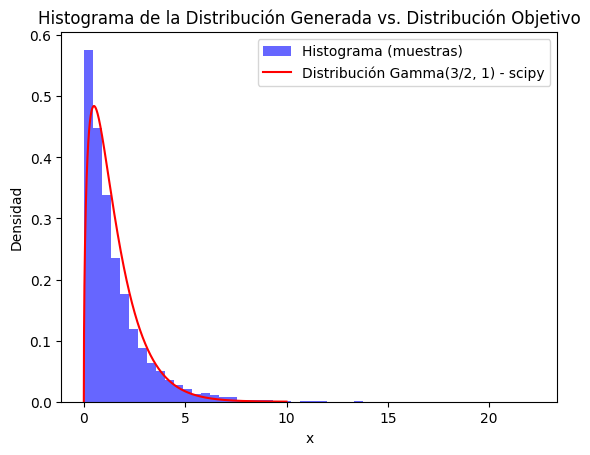
\includegraphics[width=0.8\textwidth]{assets/gamma.png}
	\caption{Histograma de la la gama simulada}
\end{figure}


\subsection{Estime $E[X^2]$ y construya la gráfica de la convergencia de los running means.}

\[
	\begin{split}
		E[X^2] & = \alpha(\alpha + 1)\beta^2      \\
		       & = \frac{3}{2}(\frac{3}{2}1)=3.75
	\end{split}
\]
\begin{pythonbox}[title={The }]
	\inputminted{python}{code/test.py}
\end{pythonbox}

\begin{figure}[H]
	\centering
	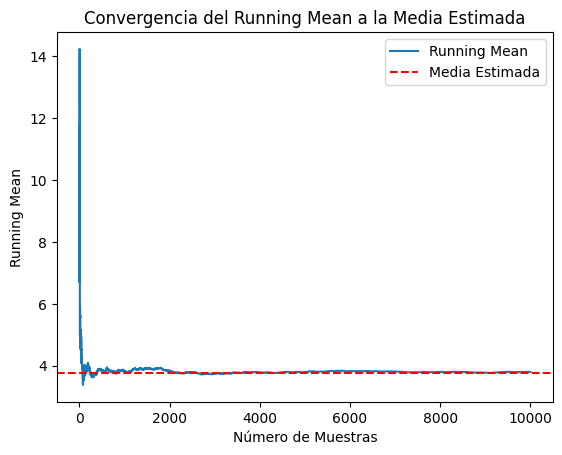
\includegraphics[width=0.8\textwidth]{assets/gama_sum.png}
	\caption{Histograma de la variable aleatoria}
\end{figure}

\section{Importance Sampling}

Usando Importance Sampling estime $E_f\left[ \frac{X^5}{1+(X - 3)^2}I[X \ge 0] \right]$, donde $f$ es la
distribución $t$ con $v=12$ Utilice las siguientes $g$:

\subsection{Estimador importance Sampling}
Para cada una de estas distribuciones presente el estimador que corresponde a la sumatoria definida
por el método de \textbf{Importance Sampling} y que converge al valor esperado de interés
\subsubsection{$Cauchy(0,1)$}
\[
	\begin{split}
		E_f\left[\frac{f(x)}{g(x)}p(x)\right] & = \frac{1}{N}\sum_{i=1}^{N}\frac{f(x)}{g(x)}p(x) ; \text{where } x \sim cauchy(0,1)                             \\
		                                      & = \frac{1}{N}\sum_{i=1}^{N}\frac{\frac{X^5}{1+(X - 3)^2}I[X \ge 0] }{\frac{1}{\pi (1 + x^2)}} \cdot student(12)
	\end{split}
\]
\subsubsection{$Normal(0, \frac{v}{v-2})$}
\[
	\begin{split}
		E_f\left[\frac{f(x)}{g(x)}p(x)\right] & = \frac{1}{N}\sum_{i=1}^{N}\frac{f(x)}{g(x)}p(x) ; \text{where } x \sim normal(0,\frac{12}{12-2}) \\
		                                      & = \frac{1}{N}\sum_{i=1}^{N}\frac{\frac{X^5}{1+(X - 3)^2}I[X \ge 0] }{}student(12)
	\end{split}
\]
\subsubsection{$Exponencial(\lambda=1)$}
\[
	\begin{split}
		E_f\left[\frac{f(x)}{g(x)}p(x)\right] & = \frac{1}{N}\sum_{i=1}^{N}\frac{f(x)}{g(x)}p(x) ; \text{where } x \sim exponential(1) \\
		                                      & = \frac{1}{N}\sum_{i=1}^{N}\frac{\frac{X^5}{1+(X - 3)^2}I[X \ge 0] }{g(x)}student(12)
	\end{split}
\]


\subsection{Estimador Monte Carlo}
Para cada uno presente el estimador que corresponde a la sumatoria definida por el método de Integración
Monte Carlos y que converge al valor esperado de interés.
\[
	\begin{split}
		MC & = \frac{1}{N}\sum_{i=1}^{N}f(x) ; \text{where } x \sim student(12) \\
		   & = \frac{1}{N}\sum_{i=1}^{N}f\frac{X^5}{1+(X - 3)^2}I[X \ge 0]
	\end{split}
\]


\subsection{Implementación}

\subsubsection{Código para Monte Carlos}
\begin{pythonbox}[Implementacion de Monte Carlos]
	\inputminted{python}{code/mc.py}
\end{pythonbox}

\subsubsection{Código para $Cauchy(0,1)$}
\begin{pythonbox}[Implementacion de distribución cauchy]
	\inputminted{python}{code/cauchy.py}
\end{pythonbox}

\subsubsection{Código para$Normal(0, \frac{v}{v-2})$}
\begin{pythonbox}[Implementacion de distribución normal]
	\inputminted{python}{code/normal.py}
\end{pythonbox}

\subsubsection{Código para $Exponencial(\lambda=1)$}
\begin{pythonbox}[Implementacion de distribución Exponencial]
	\inputminted{python}{code/exp.py}
\end{pythonbox}

\subsection{Gráficas}
Construya un asola gracia y presente la convergencia de los running menas para los cuatro estimadores. Compare la varianza empírica de los
cuatro estimadores

\begin{pythonbox}[Implementacion de distribución Exponencial]
	\inputminted{python}{code/all_graphs.py}
\end{pythonbox}


\begin{figure}[H]
	\centering
	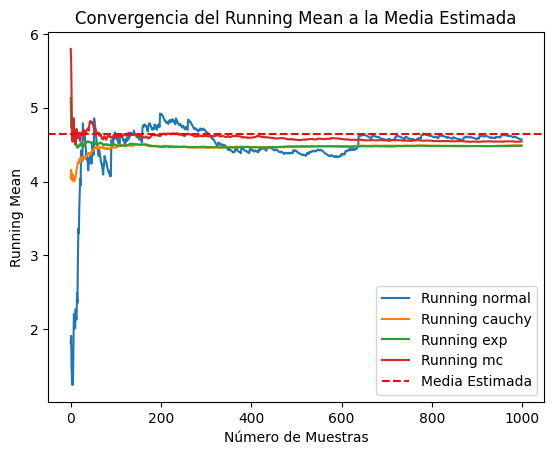
\includegraphics[width=0.8\textwidth]{assets/graph.png}
	\caption{Histograma de la variable aleatoria}
\end{figure}

\end{document}
